\section{Reading In}
\label{sec:lit}

A topic chosen is a literature owed.
Our lit-review rules are few enough to fit in a box:
Figure~\ref{fig:prompt} shows the whole prompt, whose first three
lines are machine-read configuration and whose rules drive the
pipeline.

\begin{figure}[t]
\fbox{\parbox{\dimexpr\linewidth-2\fboxsep-2\fboxrule}{\small
{\ttfamily goal:~~human factors of AI assistants\\ \hspace*{4.2em}for
[software engineering]\\ years:~2021-2026\\ seed:~~(one anchor DOI per
wing)}\\[0.4em] Rules: (1)~define ``recent'' by field velocity: ten
years default, two to three for LLM-speed fields; (2)~the bracketed
goal term is a venue filter: the initial grab searches only inside
that field's venues, per a reviewable venue list;\footnote{Sources for
the list: se-deadlines.github.io, Google Scholar's venue index for
``software engineering'', OpenAlex sources whose names contain
``software'', and the venues of the team's own recent papers.
CORE no longer lists journals.}
(3)~sort the hits by citations and read above the knee of that curve
(the point farthest from the first-to-last chord); (4)~seeds join the
reading set regardless of the knee; (5)~snowballing is unrestricted:
backward from the reading set for the classics and forward from the
seeds for the newest work, roaming outside the field on purpose;
(6)~the download rate is a finding: report it, never silently drop
missing papers.
Then code every abstract; hunt for subsets and their overlaps; and
list which of the team's own papers already sit inside the set.}}
\caption{The prompt that runs the literature review
(from the rite engine's search rules, github.com/timm/rite).}
\label{fig:prompt}
\end{figure}

\begin{figure}[t]
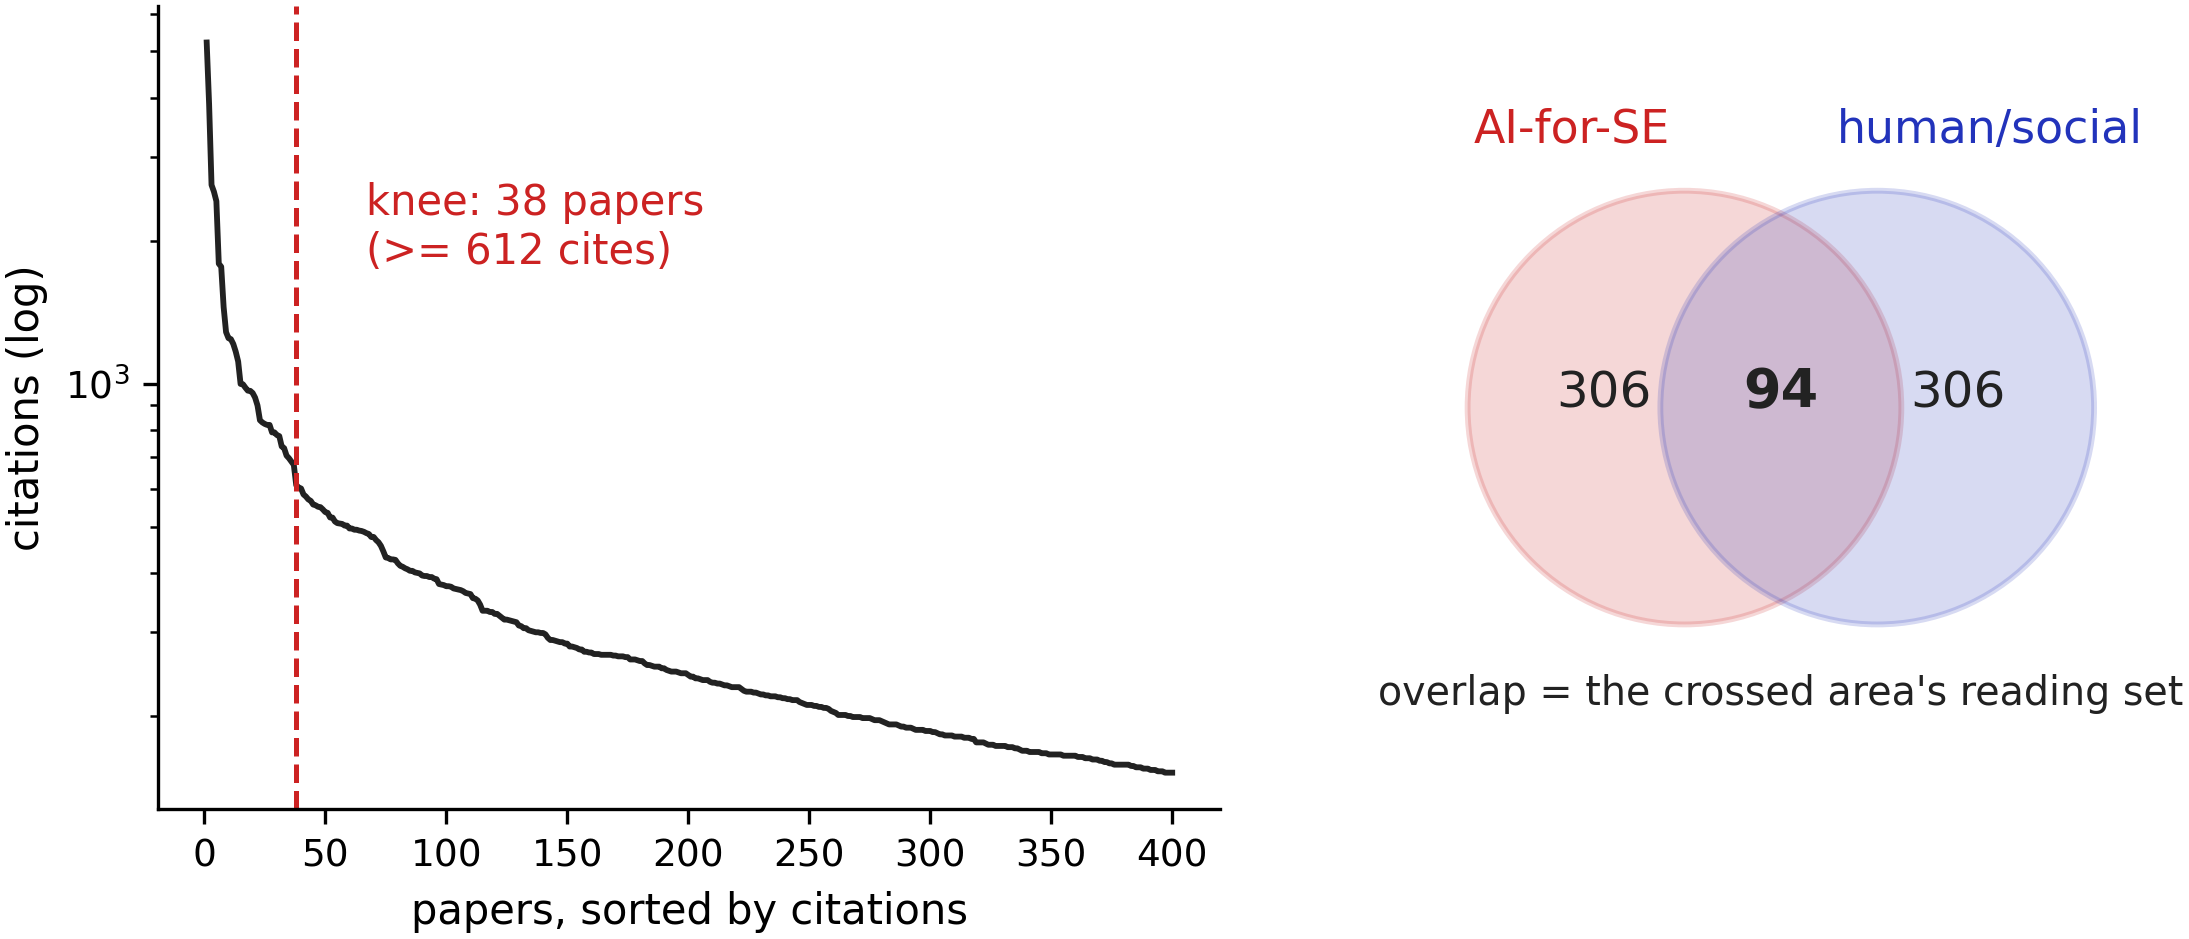
\includegraphics[width=\linewidth]{fig/lit}
\caption{Left: the sorted-cites curve of the goal
query, searched within SE venues only (\litSE{} papers, OpenAlex,
2021--2026).
The dotted line joins the most- to the least-cited paper; the dashed
drop marks the point farthest from that line, i.e.\ the knee:
\litKnee{} papers at \litKneeCites{} citations or more.
Right: the two wings as separate queries, same venues; their
\litBoth-paper overlap.
Regenerate via {\em litfig.py}.}
\label{fig:lit}
\end{figure}

Figure~\ref{fig:lit} shows the rules running on the area that
\S\ref{sec:map} chose.
The venue rule earned its place twice.
A first draft of this section skipped it, and the reading set filled
with general AI blockbusters (a machine learning survey, the GPT-4
report, a metaverse position paper) from venues nowhere near software
engineering.
A second draft filtered venues after a citation-sorted fetch, and that
failed too: of the top 1{,}000 hits, only nine sat in SE venues, since
mega-cited outsiders crowd out the field long before the filter runs.
Hence the venue list joins the query itself, and the human hours are
spent only on papers our field would recognize.

\begin{figure}[t]
\centering
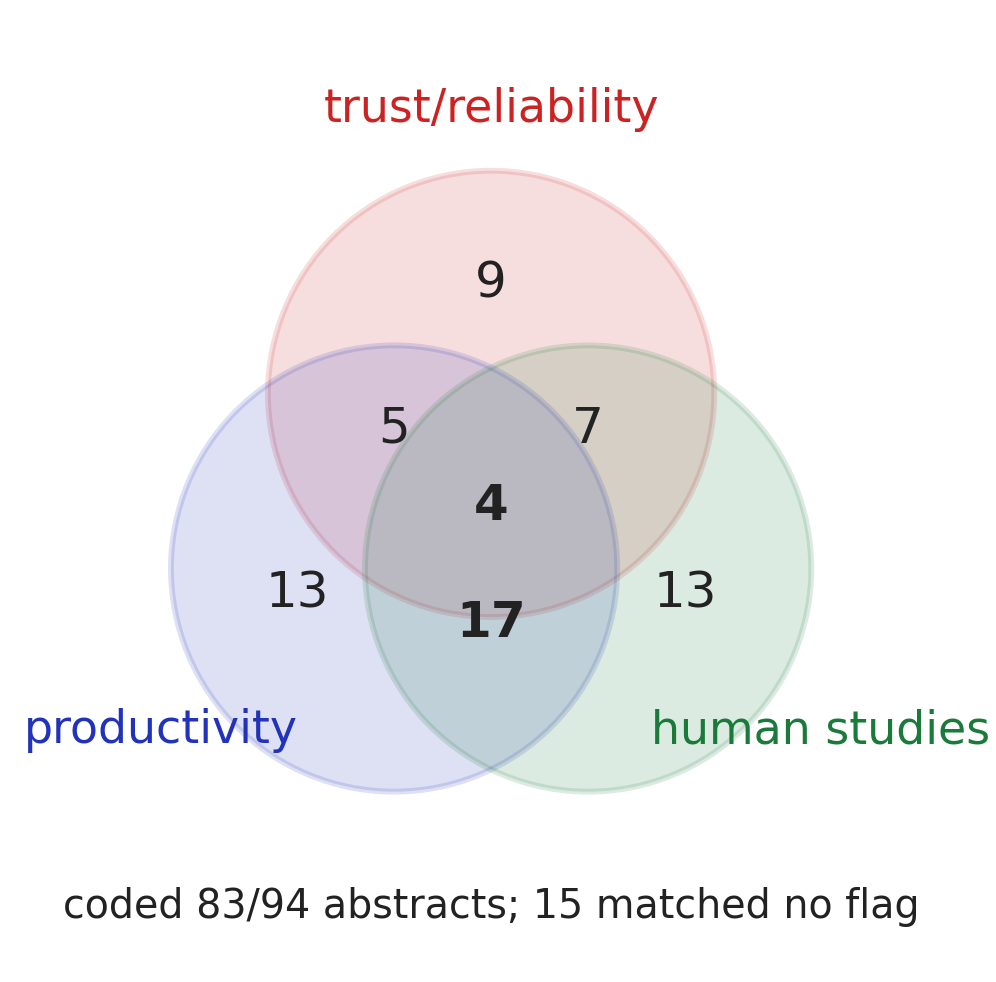
\includegraphics[width=0.62\linewidth]{fig/lit2}
\caption{The reading set (\litRead{} papers: the
\litKnee{} above the knee of Figure~\ref{fig:lit}, plus three seeds),
coded against three topic flags.
Regenerate via {\em litfig.py}.}
\label{fig:lit2}
\end{figure}

The reading set is what sits above the knee, plus the seeds that
rule~(4) admits regardless of citations: \litRead{} papers in all, of
which \litAbs{} had retrievable abstracts.
Here the seeds are the team's own three in-query papers (rows marked
``s'' in Table~\ref{tab:read}).
Figure~\ref{fig:lit2} codes those with three topic flags (trust,
productivity, human-method); \litTPH{} papers occupy all three
circles, and \litNone{} match no flag.
Table~\ref{tab:read} lists the reading set itself, with its flags.

\begin{table*}[t]
\caption{The reading set: title (first author), venue,
year, citations, and the three topic flags of Figure~\ref{fig:lit2}.
Rows marked ``s'' are seeds: the team's own in-query papers,
admitted regardless of the knee.
Generated by {\em litfig.py} from OpenAlex; venues as recorded there.}
\label{tab:read}
\scriptsize \setlength{\tabcolsep}{3pt}
\centering
% generated by litfig.py; do not hand-edit
\begin{tabular}{@{}rp{0.58\linewidth}p{0.17\linewidth}rr@{}}
\toprule
\# & paper & venue & year & cites\\
\midrule
1 & Machine Learning: Algorithms, Real-World Application... (Sarker) & SN Computer Science & 2021 & 5221\\
2 & Opinion Paper: “So what if ChatGPT wrote it?” Multid... (Dwivedi) & International Journal  & 2023 & 3869\\
3 & Metaverse beyond the hype: Multidisciplinary perspec... (Dwivedi) & International Journal  & 2022 & 2619\\
4 & Machine learning and deep learning (Janiesch) & Electronic Markets & 2021 & 2534\\
5 & GPT-4 Technical Report (OpenAI) & arXiv (Cornell Univers & 2023 & 2421\\
6 & A Metaverse: Taxonomy, Components, Applications, and... (Park) & IEEE Access & 2022 & 1789\\
7 & Natural language processing: state of the art, curre... (Khurana) & Multimedia Tools and A & 2022 & 1762\\
8 & ARTIFICIAL INTELLIGENCE FOR THE REAL WORLD (?) & International Research & 2023 & 1450\\
9 & A survey on large language model based autonomous ag... (Wang) & Frontiers of Computer  & 2024 & 1284\\
10 & Flamingo: a Visual Language Model for Few-Shot Learn... (Jean-Baptiste) & arXiv (Cornell Univers & 2022 & 1247\\
11 & Generative AI (Feuerriegel) & Business \& Informatio & 2023 & 1241\\
12 & A SWOT analysis of ChatGPT: Implications for educati... (Farrokhnia) & Innovations in Educati & 2023 & 1212\\
13 & A Review of Artificial Intelligence (AI) in Educatio... (Zhai) & Complexity & 2021 & 1168\\
14 & AI-Based Modeling: Techniques, Applications and Rese... (Sarker) & SN Computer Science & 2022 & 1114\\
15 & Hydrogen production, storage, utilisation and enviro... (Osman) & Environmental Chemistr & 2021 & 999\\
16 & Deep learning modelling techniques: current progress... (Ahmed) & Artificial Intelligenc & 2023 & 997\\
17 & The future landscape of large language models in med... (Clusmann) & Communications Medicin & 2023 & 981\\
18 & Unmanned aerial vehicles (UAVs): practical aspects, ... (Mohsan) & Intelligent Service Ro & 2023 & 967\\
19 & A Survey on the Explainability of Supervised Machine... (Burkart) & Journal of Artificial  & 2021 & 966\\
20 & New Era of Artificial Intelligence in Education: Tow... (Kamalov) & Sustainability & 2023 & 956\\
21 & Artificial intelligence and smart vision for buildin... (Baduge) & Automation in Construc & 2022 & 935\\
22 & Using machine learning approaches for multi-omics da... (Reel) & Biotechnology Advances & 2021 & 900\\
23 & A Review of the Role of Artificial Intelligence in H... (Kuwaiti) & Journal of Personalize & 2023 & 838\\
24 & Unlocking the value of artificial intelligence in hu... (Chowdhury) & Human Resource Managem & 2022 & 829\\
25 & A survey on deep learning tools dealing with data sc... (Alzubaidi) & Journal Of Big Data & 2023 & 823\\
26 & Smart wearable devices in cardiovascular care: where... (Bayoumy) & Nature Reviews Cardiol & 2021 & 819\\
27 & Adaptive Learning Using Artificial Intelligence in e... (Gligorea) & Education Sciences & 2023 & 819\\
28 & <scp>ChatGPT</scp> and a new academic reality: <scp>... (Lund) & Journal of the Associa & 2023 & 790\\
29 & Human resource management in the age of generative a... (Budhwar) & Human Resource Managem & 2023 & 790\\
30 & Challenges and Opportunities of Generative AI for Hi... (Michel‐Villarreal) & Education Sciences & 2023 & 780\\
31 & Survey on 6G Frontiers: Trends, Applications, Requir... (Alwis) & IEEE Open Journal of t & 2021 & 776\\
32 & A Review on Large Language Models: Architectures, Ap... (Raiaan) & IEEE Access & 2024 & 738\\
33 & AI Tools in Society: Impacts on Cognitive Offloading... (Gerlich) & Societies & 2025 & 732\\
34 & Academic Integrity considerations of AI Large Langua... (Perkins) & Journal of University  & 2023 & 706\\
35 & ChatGPT and Open-AI Models: A Preliminary Review (Roumeliotis) & Future Internet & 2023 & 697\\
36 & Retrieval-Augmented Generation for Large Language Mo... (Gao) & arXiv (Cornell Univers & 2023 & 686\\
37 & The impact of big data analytics and artificial inte... (Benzidia) & Technological Forecast & 2021 & 675\\
38 & Teachers’ AI digital competencies and twenty-first c... (Ng) & Educational Technology & 2023 & 612\\
\bottomrule
\end{tabular}

\end{table*}

Snowballing then ran from that set, deliberately unfiltered by venue,
since good ancestors and good critics live anywhere: backward
collection found \litRefs{} distinct references (\litClassics{} cited
by two or more of the reading set: the candidate classics); forward
collection found \litCiting{} works already citing the reading set.
\note{timm}{the three flags are paper0-local; a full run would fork
its own workdir and flags.py, per the engine rules}

The process itself yielded findings worth recording.
Full texts are scarce: in this workdir's companion pipeline run, only
22 of 54 chased PDFs (41\%) could be downloaded; abstracts come easier
(here, \litAbs{} of \litKnee).
Google Scholar is closed to scripts; OpenAlex, Semantic Scholar, and
arXiv answer machine queries gladly, so the pipeline builds only on
the willing.
An earlier full-text pass showed abstract-only coding missing about
half the flags; hence full text is coded above the knee.
Finally, the own-papers rule paid off: \litOwn{} papers by this team
(Di Nucci on accessibility, Schmid on MLOps, Esposito on AI agents)
already sit in the venue-filtered goal results.
The territory is adjacent to us without yet being occupied by us.

Reading done, the loop starts writing.
Figure~\ref{fig:sample} shows what that looks like: the step-8 draft
(title, elevator speech, abstract, questions, contributions) plus the
step-9 lit-review pivot, generated for the very topic that
\S\ref{sec:map} nominated, then frozen here as an exhibit rather than
polished into a claim.

\begin{figure*}[b!]
\fbox{\begin{minipage}{\dimexpr\textwidth-2\fboxsep-2\fboxrule}
\small
\begin{center}
{\scshape\bfseries Example output (synthetic)}\\[0.1em]
{\footnotesize What the loop emits at step 8 for the topic
nominated in \S\ref{sec:map}; unedited machine draft, before the
critics of steps 10--14. Nothing here is a measured claim of this
paper.}
\end{center}
\vspace{0.3em}
\begin{minipage}[t]{0.47\textwidth}
\textbf{paper[0]: title, elevator speech, abstract.}\\[0.3em]
{\em Do AI Assistants Amplify or Erase a Team's Measured
Strengths?}\\[0.4em]
\begin{quote}
Six researchers, measured from their own corpus, split into a wing
that measures and a wing that crafts.
When LLM assistants join the loop, does the work drift toward those
peaks, or toward the model's mean?
We propose an instrument that answers this per team, in minutes,
from public records.
\end{quote}
{\em Abstract:} Teams adopt LLM writing assistants faster than they
can measure the effect on their own output.
We reverse engineer a team's strengths from its published corpus
(repertory grid over coded papers, FOCUS sorted), instrument one
year of assisted and unassisted writing, and measure drift between
the two against the team's own baseline.
The instrument runs from public records in minutes.
Scripts, data, and grids: github.com/timm/how2rite.
\end{minipage}\hfill
\begin{minipage}[t]{0.47\textwidth}
\textbf{Research questions} (answers land inline, in bold, once
step 9's experiments run).\\
RQ1: Can a team's strengths be recovered from its public corpus
alone?\\
RQ2: Does assisted output sit nearer the team's measured centroid,
or the model's default register?\\
RQ3: Which member-to-area pairings does the drift evidence
support?\\[0.5em]
\textbf{Contributions.}
(1)~a corpus-derived strengths instrument (grid plus FOCUS sort);
(2)~a measured map of six researchers against the nine ICSE'27
areas;
(3)~blend arithmetic that nominates cross-wing topics;
(4)~a replication package: github.com/timm/how2rite.\\[0.5em]
\textbf{Step 9, the lit-review pivot} (form: respect, then
disrespect, then the open-issues list).\\[0.3em]
Prior work earns respect on two fronts: trust in AI assistants is
now measured at the level of the individual developer, and
productivity effects are quantified across thousands of sessions.
However, the corpora end where teams begin: the trust studies
observe single subjects, and the productivity numbers average away
exactly the between-member differences that define a team.
Based on the above, three issues remain open: (i)~team-level
measures of strength, (ii)~drift of assisted output against such
measures, and (iii)~longitudinal designs that separate tool effects
from team learning.
The sections that follow address (i) and (ii); issue (iii) is
future work.
\end{minipage}
\end{minipage}}
\caption{A worked sample of the loop's own prose products, boxed
and labeled so no reader mistakes it for a result.
The form follows the engine's structure rules (github.com/timm/rite):
question-form title without hyphens, elevator speech in a quote
block, research questions answered inline, contributions ending in
the replication URL, and a lit review that pivots on its
open-issues list.}
\label{fig:sample}
\end{figure*}

\begin{pause}{the search}
Ask: are the goal line and the two wing queries the right words?
Is 2021 the right floor for ``recent''?
Is the venue list (see the box) the SE you mean, and are the three
coding flags the vocabulary you would use?
Is a knee that keeps \litKnee{} of \litSE{} papers too
greedy?\\[0.2em] To change the outcome: edit the query strings,
{\ttfamily VENUES}, and {\ttfamily FLAGS} in {\ttfamily litfig.py},
delete the cache in {\ttfamily tmp/}, and rerun; both figures, the
table, and every number in this section regenerate.
\end{pause}
